\chapter{Integration Into Machine Translation Systems}
\label{chap:integration}
In this chapter, we demonstrate how our CL-WSD techniques can be integrated
into running machine translation systems, with the goal of improving lexical
selection in practice, while minimizing code changes to the MT software. We
translate from Spanish to Guarani with Moses\cite{koehn-EtAl:2007:PosterDemo},
an off-the-shelf phrase-based statistical MT system, and from Spanish to
Quechua with SQUOIA, a rule-based MT system that was developed by Rios \emph{et
al.} at the University of Zürich. These two integrations are meant to be simple
proofs of concept, rather than an attempt to define a best practice, but they
demonstrate at least conceptually how CL-WSD can be used with these translation
systems.  Afterwards, we look at evaluating Chipa's effect on MT output in both
of these use cases.

Among other pieces of software related to this work, especially the corpus
preparation scripts, the code to integrate Chipa into these machine
translation systems is in a package called Tereré \footnote{Available at
\url{http://github.com/alexrudnick/terere} ; Tereré is a cold variety of yerba
mate brewed with ice water; it is a specifically Paraguayan specialty.}.

\section{Integrating Chipa into Phrase-Based Statistical Machine Translation}
Moses\footnote{Available at
\url{http://statmt.org/moses/}} is a mature,
well-maintained and popular statistical machine translation package, in broad
use for both research and practical purposes. Conveniently for our work here,
it includes an interface for adding feature functions\footnote{See
\url{http://www.statmt.org/moses/?n=Moses.FeatureFunctions} for documentation.}
to guide its decoding process.

Moses, like many SMT systems, combines signals from different subcomponents
when searching through the space of possible translations. It does this using a
log-linear model, in which each component scores a candidate translation, and
then the scores from the different components are combined with a weighted sum.
Some typical components are the probabilities learned for a given phrase during
phrase extraction (without regard to context) in both translation directions,
scores from the target-language language model, learned distortion models that
reflect estimated differences in word order between source and target
languages, and a handful of other features\footnote{For an overview of
techniques commonly used in phrase-based statistical MT, please see Koehn's
book on the subject \cite{koehn2010statistical}.}. The weights for each
subcomponent are typically tuned with Minimum Error-Rate Training, or ``MERT"
\cite{och:2003:ACL}.

Scores in this framework are expected to represent log probabilities, meaning
that, concretely, they are real numbers less than 0, as the logarithm of a
number between 0 and 1 will be negative. The beam search procedure then
attempts to maximize the total score for a translation, which means finding a
translation with a score as high as possible, \emph{i.e.}, maximally close to
0.

We built a simple phrase-based SMT system with Moses and used this feature
function API to have Chipa evaluate candidate translations.
For simplicity, we added a constraint in the Moses phrase-extraction system
so that the source side of all phrases must be at most one token long, to match
the alignments used in the previous chapters.

During the search through the space of possible translations, Moses proposes
candidate translations for each source word to Chipa ...
which provides a score based on how likely the translation seems to the CL-WSD
system, based on the entire source-language sentence context. This score is
returned to Moses, which combines all of the available features in a log-linear
combination.

The weights for all of the features provided to the system (translation
probabilities, LM scores, CL-WSD scores, and perhaps others) can be tuned on a
development set with MERT \cite{och:2003:ACL}; thus, if CL-WSD scores turn out
to be useful for achieving high BLEU scores on the development set sentences,
Chipa's feature function will be assigned a higher weight. If not, its advice
carries less weight, than, for example, that of the language model.


\subsection{Interfacing between Moses and Chipa}
%% write about how we can't we just annotate the phrase table for individual
%% sentences just before decoding -- we need to know about the phrase *in a
%% context* and that's the point.
We implemented a simple protocol for communication between the Moses C++ code
and the Chipa server, based on Unix pipes; see Figure
\ref{fig:moses-chipa-diagram} for a visual aid. In earlier work with SQUOIA
\cite{rudnick:saltmil2014}, we had communicated between Chipa and the machine
translation system with XML-RPC \footnote{\url{http://xmlrpc.scripting.com/}},
but for simplicity of implementation, we built a simpler text-based protocol.

Named Unix pipes, or FIFOs, allow the creation of a special kind of filesystem
object whereby messages can be passed between processes in the same computer.
Here Moses requests an evaluation for a certain translation of a
source-language phrase, and Chipa returns a score based on how likely it
considers that phrase, represented as log probabilities. 

\begin{figure}
  \begin{centering}
  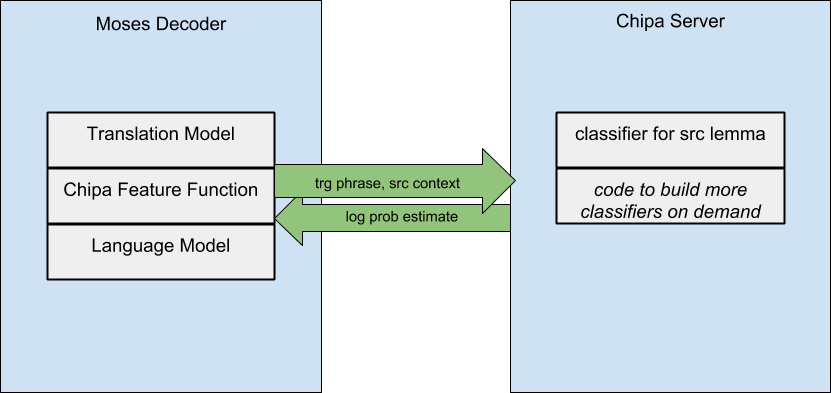
\includegraphics[width=15cm]{moses-chipa-diagram.png}
  \end{centering}
  \caption{Schematic diagram showing the relationship between the Moses decoder
  process, running the custom-made Chipa feature function, which communicates
  with the Chipa server process. The Chipa server returns probability
  estimates for proposed target-language phrases based on the given
  source-sentence context, when available.}
  \label{fig:moses-chipa-diagram}
\end{figure}

\section{Integrating Chipa into Rule-Based Machine Translation}


\subsection{The SQUOIA RBMT system}
SQUOIA\footnote{Code available at \url{https://github.com/a-rios/squoia} ;
the project is more broadly described at
\url{https://www.cl.uzh.ch/en/research/machine-translation/hybridmt.html}}
is a project for rule-based machine translation from Spanish to Quechua.

SQUOIA was developed by a team at the University of Zurich. For the most
part, it is a classical rule-based transfer system, although the team has
developed techniques for predicting verb morphology with machine
learning methods, in cases when rules cannot reliably disambiguate
\cite{riosgonzales-gohring:2013:HyTra}. It does not, by default, use machine
learning for lexical selection as such, although it does include a language
model to select among the licensed alternatives.

SQUOIA's architecture is based on the Matxin system \cite{matxin2005}, which
was originally intended for translating from Spanish to Basque.
It consists of a pipeline of smaller steps, each of which passes along a tree
describing the current input sentence, in XML form. Adding CL-WSD to this
system involves adding a step to the pipeline that interprets the XML
representation of the current sentence, constrains the lexical choices based on
the recommendations of the Chipa software, and then passes these choices to
subsequent scripts.

The core system relies on a classical transfer approach and is mostly
rule-based, with a few components based on machine learning.

Each module performs some transformation on its input and
passes along the updated version to the next stage. Many modules focus on very
particular parts of the representation, leaving most of their input unchanged.

Rios and G\"{o}hring \cite{riosgonzales-gohring:2013:HyTra} describe
earlier work on extending the SQUOIA MT system with machine learning modules.

Lexical ambiguity is a significant problem facing rule-based machine
translation systems, as many words have several possible translations in a
given target language, each of which can be considered a sense of the word from
the source language.

The difficulty of resolving these ambiguities is mitigated for 
statistical machine translation systems for language pairs with large bilingual
corpora, as large n-gram language models and phrase tables containing common
multi-word expressions can encourage coherent word choices.
For most language pairs these resources are not available, so a primarily
rule-based approach becomes attractive.

In cases where some training data is available, though, we can
investigate hybrid RBMT and machine learning approaches, leveraging small and
potentially growing bilingual corpora.

... show how it allows us to learn from the available bitext to
make better lexical choices, with very few code changes to the base system.

The integration enables SQUOIA to take advantage of any available bitext
without significantly changing its design, and to improve its word choices as
additional bitext becomes available.

In its current design, SQUOIA makes word choices based on its bilingual
lexicon; the possible translations for a given word or multi-word expression
are retrieved from a dictionary on demand. If there are several possible
translations for a lexical item, these are passed along the pipeline so
that later stages can make a decision, but if the ambiguity persists,
then the first entry retrieved from the lexicon is selected. While there are
some rules for lexical selection, they have been written by hand and only cover
a small subset of the vocabulary in a limited number of contexts.

In this work, we supplement these rules with classifiers learned from
Spanish-Quechua bitext.  These classifiers make use of regularities that may not
be obvious to human rule-writers, providing improved lexical selection for
any word type that has adequate coverage in the training corpus.

There are many dialects of Quechua; SQUOIA focuses on the
Cuzco dialect, spoken around the Peruvian city of Cuzco.

In the first stages, Spanish source sentences are analyzed with off-the-shelf
open-source NLP tools. To analyze the input Spanish text,
SQUOIA uses FreeLing \cite{padro12} for morphological analysis and named-entity
recognition,
Wapiti \cite{lavergne2010practical} for tagging,
and DeSr \cite{attardi-EtAl:2007:EMNLP-CoNLL2007} for parsing.
All of these modules rely on statistical models.

In the next step, the Spanish verbs must be disambiguated in order to assign
them a Quechua verb form for generation: a rule-based module tries to assign a
verb form to each verb chunk based on contextual information. If the rules fail to
do so due to parsing or tagging errors, the verb is marked as ambiguous and
passed on to an SVM classifier, which assigns a verb form even if the context
of that verb does not unambiguously select a target form. This is among the
most difficult parts of the
translation process, as the grammatical categories encoded in verbs differ
substantially between Spanish and Quechua. In the next step, a lexical transfer
module inserts all possible translations for every word from a bilingual dictionary.
Then a set of rules disambiguates the forms with lexical or morphological
ambiguities. However, this rule-based lexical disambiguation is very limited,
as it is not feasible to cover all possible contexts for every ambiguous word
with rules.

The rest of the system makes use of a classical transfer procedure. A following module
moves syntactic information between the nodes and the chunks in the tree, and
finally, the tree is reordered according to the basic word order in the target
language. In the last step, the Quechua surface forms are morphologically
generated through a finite state transducer.

In order to integrate Chipa into SQUOIA, we added an additional lexical
selection stage to the SQUOIA pipeline, occurring after the rule-based
disambiguation modules, but before a number of other steps. This new module
examines the XML tree structure of a SQUOIA translation in progress, and finds
nodes in the tree where there are several possible Quechua lemmas that may be
chosen as a translation. It then extracts the surface forms and lemmas of the
input sentence from the current XML tree structure, and passes these along to
the Chipa system so that we can make a prediction as to what the correct
translation for that input token should be.

For each word with such multiple translation possibilities, we look at each of
the translations under consideration by SQUOIA, and if any of them was the top 
classification output from the Chipa classifiers, we constrain SQUOIA to take
that choice.
%% XXX: working here
If there are no such overlapping translations, we
take the default entry suggested by SQUOIA's dictionary.
Notably, since Chipa and SQUOIA do not share the same lexicon and bitext alignments
may be noisy, translations
observed in the bitext may be unknown to the SQUOIA system, and lexical entries in the
SQUOIA dictionary may not be attested in the training data.

\section{Translation Evaluation for Spanish-Guarani}

%% TODO: explain how we sampled test sets, what it means that we picked verses
%% rather than sentences

\subsection{Results: BLEU scores for Spanish-Guarani}
\begin{figure*}
  \begin{centering}
  \begin{tabulary}{\textwidth}{|R|L|}
    \hline
    setting & BLEU \\
    \hline
    Moses with Chipa enabled &  16.24 \\
    \hline
    Same system, with Chipa disabled &  10.01 \\
    \hline
  \end{tabulary}
  \end{centering}
  \caption{BLEU scores on our Spanish-Guarani test set. Note that this is
  translating to \emph{lemmatized} Guarani, rather than having to predict
  fully-inflected forms.}
  \label{fig:pyramid-extras-results}
\end{figure*}


\section{Translation Evaluation for Spanish-Quechua}

In order to evaluate the effect of Chipa on lexical selection in a live
translation task, we used SQUOIA to translate a hundred verses sampled from our
Spanish-Quechua Bible bitext, both in its default settings, and with the
addition of Chipa. The BLEU scores for SQUOIA output on this test set were
quite low (lower than one BLEU point), and were not improved by adding the
Chipa CL-WSD, but this is a rather more difficult task, since we are attempting
to generate fully-inflected Quechua surface forms, rather than selecting
appropriate lemmas.

In any case, here we will show examples of word choices that were changed with
the addition of Chipa CL-WSD, and, armed with our Spanish-Quechua dictionary
\cite{academiamayor}, determine whether they are more or less appropriate than
the choices that the SQUOIA system would have made on its own.


One pattern that we find is that Chipa tends to encourage SQUOIA to choose
\emph{churi} (a son, when discussed with regard to his father) rather than the
more generic \emph{wawa}, which can refer to any child; in all of the test
sentences where we saw this choice happen, it was an appropriate choice.

But more generally, we see some good word choices... XXX


For example, we see when translating Sentence \ref{sent:alreadydead} (``Pilate
was surprised that he had already died, and calling the centurion, asked him if
he was already dead.") from Spanish to Quechua, without Chipa, SQUOIA
translates \emph{llamando} ('calling') to \emph{sutikuspa}, where \emph{suti}
is the sense of ``llamar" that refers to naming. However, with Chipa, SQUOIA
picks \emph{waqyaspa}, where \emph{waqyay} is the communicative sense, rather
than the naming sense.

\begin{figure*}
\enumsentence{
Pilato se sorprendió de que ya hubiera muerto, y llamando al centurión, le
preguntó si ya estaba muerto.}
\label{sent:alreadydead}

\enumsentence{
Jehová dijo a Moisés: -- Toma a Josué hijo de Nun, hombre en el cual hay
espíritu, y pon tu mano sobre él.}
\label{sent:putyourhand}

  \caption{Selected Spanish passages for which adding Chipa generated different
  Quechua translations}
  \label{fig:some-spanish-verses-with-changes}
\end{figure*}
